\documentclass[a4paper]{article}
\usepackage[utf8]{inputenc}
\usepackage[margin=1in, footskip=0.25in]{geometry}

\usepackage{graphicx}
\graphicspath{../}

\usepackage{booktabs}
\usepackage{wrapfig}

\usepackage[backend=bibtex, style=numeric, sorting=none]{biblatex}
\bibliography{references}
%\addbibresource{references.bib}

\usepackage[font=footnotesize,labelfont=bf]{caption}
\captionsetup{width=\columnwidth}

\usepackage{amsmath}

\begin{document}
	
	% ======================= start titlepage ==============================================
	
	\begin{titlepage}
		\begin{center}
			\Large Numerical Methods in Astrophysics \\
			\vspace{1cm}
			\huge{
				Project 2 \\
				\vspace{0.5cm}
				\textbf{Ordinary Differential Equations,}\\
				\textbf{Fourier Transforms and} \\
				\textbf{Spectral Analysis} \\
				\vspace{1cm}
			}
			\Large \emph{Saksham Kaushal}
		\end{center}
	\end{titlepage}
	
	% =========================end titlepage ================================================
	
	\tableofcontents
	\newpage
	
	% ========================= Introduction ================================================
	
	\section{Introduction} \label{Introduction}
	% Description of Physical scenario
	
	% ========================= Part 1 ======================================================
	
	\newpage
	\section{Part 1 - Ordinary Differential Equations} \label{task1}
	
	For stars in disk of the galaxy, equation of motion is given by equation 19 of the lecture notes as,
	\begin{equation}
		\frac{d^2r(t)}{dt^2} = - \nabla \Phi (r) -2 \Omega_B \times v+ \Omega_B^2 r ,
		\label{eq:motion1}
	\end{equation}
	
	where \(\Omega_B\) is angular velocity and the gravitational potential, \(\Phi (r)\) in the two dimensions for an elongated bar structure is given by equation 20 of lecture notes as,
	\begin{equation}
		\Phi(x,y)=\frac{v_0^2}{2} ln(a^2+x^2+\frac{y^2}{q^2}). 
		\label{eq:grav_potential}
	\end{equation}
	
	The gradients of gravitational potential along the two axes are given by partial derivatives of equation (\ref{eq:grav_potential}) with respect to \(x\) and \(y\) as follows,
	\begin{equation}
		\frac{\partial \Phi}{\partial x} = \frac{v_0^2 x}{a^2+x^2+\frac{y^2}{q^2}},
		\label{eq:grad_grav_potential_x}
	\end{equation}
	\begin{equation}
		\frac{\partial \Phi}{\partial y} = \frac{v_0^2 y}{q^2(a^2+x^2+\frac{y^2}{q^2})}.
		\label{eq:grad_grav_potential_y}
	\end{equation}
	
	We can substitute equations (\ref{eq:grad_grav_potential_x}) and (\ref{eq:grad_grav_potential_y}) in equation (\ref{eq:motion1}) to obtain the equation of motion that can be solved in our simulation. Equations along the two axes are given by,
	\begin{equation}
		a_x = \frac{d^2x}{dt^2} = - \frac{v_0^2 x}{a^2+x^2+\frac{y^2}{q^2}} + 2\Omega_B v_y + x \Omega_B^2 ,
		\label{eq:acceleration_x}
	\end{equation}
	\begin{equation}
		a_y = \frac{d^2y}{dt^2} = - \frac{v_0^2 y}{q^2(a^2+x^2+\frac{y^2}{q^2})} - 2\Omega_B v_x + y \Omega_B^2,
		\label{eq:acceleration_y}
	\end{equation}
	
	where it must be noted that for second term on the right hand side of equation (\ref{eq:acceleration_x}), the cross product \(\Omega_B \times v_x = -v_y\) and for similar term in equation (\ref{eq:acceleration_y}), \(\Omega_B \times v_y = v_x\), where \(\Omega_B\) has the direction perpendicularly outwards from the x-y plane.
	
	The value of \emph{Jacobi integral} is conserved as a star moves in a rotating barred potential and  therefore, minimum dispersion in its values throughout the simulation indicates better numerical integration. Its value is given by 
	\begin{equation}
		E_j \equiv \frac{\dot r^2}{2} + \Phi -\frac{(\Omega_B \times r)^2}{2}.
		\label{eq:jacobi_integral}
	\end{equation}
	
	From equation 13 of the lecture notes, the numerical error in each integration time-step can be controlled by adapting the step-size accordingly. If we define,
	\begin{equation}
		\Delta_0 \equiv \epsilon y_{max},
		\label{eq:numerical_error}
	\end{equation}
	then \(\Delta < \Delta_0\) should be satisfied for each integration step, where \(\Delta\) is the numerical error of a given step, \(\epsilon\) is the parameter defining the accuracy of integration and \(y_{max}\) is the amplitude of function in the range over which function is being integrated. If this inequality does not hold true, the values need to be adjusted accordingly, and the integration step is repeated with reduced step-size until this inequality is satisfied. However, if this inequality does indeed hold true such that \(\Delta \ll \Delta_0\), integration step-size can be safely increased to reduce the difference between \(\Delta\) and \(\Delta_0\). The step-size can be update according to equation 14 of lecture notes, given as,
	\begin{equation}
		h = h_n \left| \frac{\Delta_0}{\Delta} \right| ^m,
		\label{eq:stepsize}
	\end{equation}
	where \(h\) is the new updated step-size, \(h_n\) is the previous step-size and \(m\) is an exponent usually set to different values when increasing or decreasing the step-size, often in the range \([0.2,0.25]\). 
	
		% ----------------------------Methods -----------------------------------------------
		
		\subsection{Methods} \label{methods1}
			
		In the FORTRAN code \emph{orbit19.f}, the four elements of array \texttt{ys} represent the values of \(x\), \(v_x\), \(y\) and \(v_y\) respectively. Value of \(a\), \(q\), \(v_0\) and \(\Omega_B\) are represented by variables \texttt{a, q, v0} and \texttt{om}. The difference between the variables \texttt{x2} and \texttt{x1} indicates the time for which the simulation takes place. This is essentially different from time-step of the simulation, that depends on the value of \(\epsilon\), which parameterizes the accuracy of integration. The four elements of array \texttt{dxdy} represent the values of \(v_x\), \(a_x\), \(v_y\) and \(a_y\). The values of \(a_x\) and \(a_y\) are calculated using the equations (\ref{eq:acceleration_x}) and (\ref{eq:acceleration_y}), and encoded in the subroutine \texttt{derivs} in the code. The Jacobi integral, given by equation (\ref{eq:jacobi_integral}) is assigned the variable \texttt{ej}. \\
		
		The following methods were employed for different tasks performed for this part of the project:
		\begin{enumerate}
			
			\item The missing \textit{x} and \textit{y} components of the equation of motion for a star in barred potential well are encoded in the subroutine \texttt{derivs} of FORTRAN program \textit{orbit19.f} as, \\
			
			\noindent \texttt{dydx(2) = -y(1)*v0**2/(a**2+y(1)**2+(y(3)**2/q**2))+2*om*y(4)+y(1)*om**2}, and \\
			\texttt{dydx(4) = -y(3)*v0**2/(q**2*(a**2+y(1)**2)+y(3)**2)-2*om*y(2)+y(3)*om**2} . \\
			
			These are the \(a_x\) and \(a_y\) components, given by equations (\ref{eq:acceleration_x}) and (\ref{eq:acceleration_y}). The \(v_x\) and \(v_y\) components were already assigned to array elements \texttt{dxdy(1)} and \texttt{dxdy(3)} respectively.
			
			\item Initial parameters of the simulation for this task, along with their values and variable names in the program are mentioned in Table \ref{table:task1.2}. 
			
			\begin{table} 
				\centering
				\begin{tabular} {c c c}
					\toprule
					\textbf{Parameter} & \textbf{Variable} & \textbf{Value} \\
					\midrule
					\(\Omega_B\) (Angular velocity) & \texttt{om} & 1.0 \\
					\(v_0\) & \texttt{v0} & 1.0 \\
					\(a\) & \texttt{a} & 0.03 \\
					\(q\) & \texttt{q} & 0.8 \\
					\(t_1\) (Initial time) & \texttt{x1} & 0.0 \\
					\(t_2\) (Final time) & \texttt{x2} & 5.0 \\
					\(x\) & \texttt{ys(1)} & 0.0 \\
					\(v_x\) & \texttt{ys(2)} & -1.68 \\
					\(y\) & \texttt{ys(3)} & 0.087 \\
					\(v_y\) & \texttt{ys(4)} & 0.0 \\
					\bottomrule
				\end{tabular}
			\caption{Initial parameters of the simulation, variable names assigned to them in the FORTRAN code and their initial values set for the first simulation.}
			\label{table:task1.2}
			\end{table}
			
			\item The value of \(\epsilon\) varies the number of time-steps involved, and therefore controls the accuracy of integration. For the initial conditions given in Table \ref{table:task1.2}, simulation is run for values of \(\epsilon\) equal to \(10^{-5}, 10^{-6}, 10^{-7}, 10^{-8}\) and \(10^{-9}\). The value of Jacobi integral, defined above, is inspected for each of these values of \(\epsilon\) and plotted on a graph using Python and its associated libraries like numpy, pandas, matplotlib and seaborn. All subsequent plotting is performed in a similar manner.
			
			\item The value of variable \texttt{x2}, defining the final time of simulation, is changed from initial value of \(5.0\) to a new value of \(20.0\), keeping all other parameters unaltered. The trajectories calculated in both the cases are then plotted.
			
			\item The value of \(v_x\) assigned to array element \texttt{ys(2)} is changed to values -1.64, -1.635, -1.63, -1.58, -1.15, -0.6, -0.524 and -0.4, and the simulation is run for each of these values to obtain the corresponding trajectories which are plotted for a final time of 20.0.
			
		\end{enumerate}
		
		% ----------------------------Results -----------------------------------------------
		
		\subsection{Results} \label{results1}
		
		\begin{itemize}
			
			\item For different values of \(\epsilon\), the variations in values of Jacobi integral are plotted in figure \ref{fig:task1.3} upto a final time of 5.0. The variations are most prominent for highest and lowest values of \(\epsilon\), and least for intermediate values. Analytically, the Jacobi integral is a conserved quantity for a three-body problem in a non-inertial frame of reference. Therefore, minimum variation in its value corresponds to most accurate numerical integration, which eventually gives us the most suitable value of \(\epsilon\).
			
			From the graph in figure \ref{fig:task1.3} and using the values of standard deviations for different values of \(\epsilon\) from table \ref{table:task1.3}, we can conclude that \(\epsilon = 10^{-7}\) is the most suitable value for integration.
			
			\begin{figure} [h]
				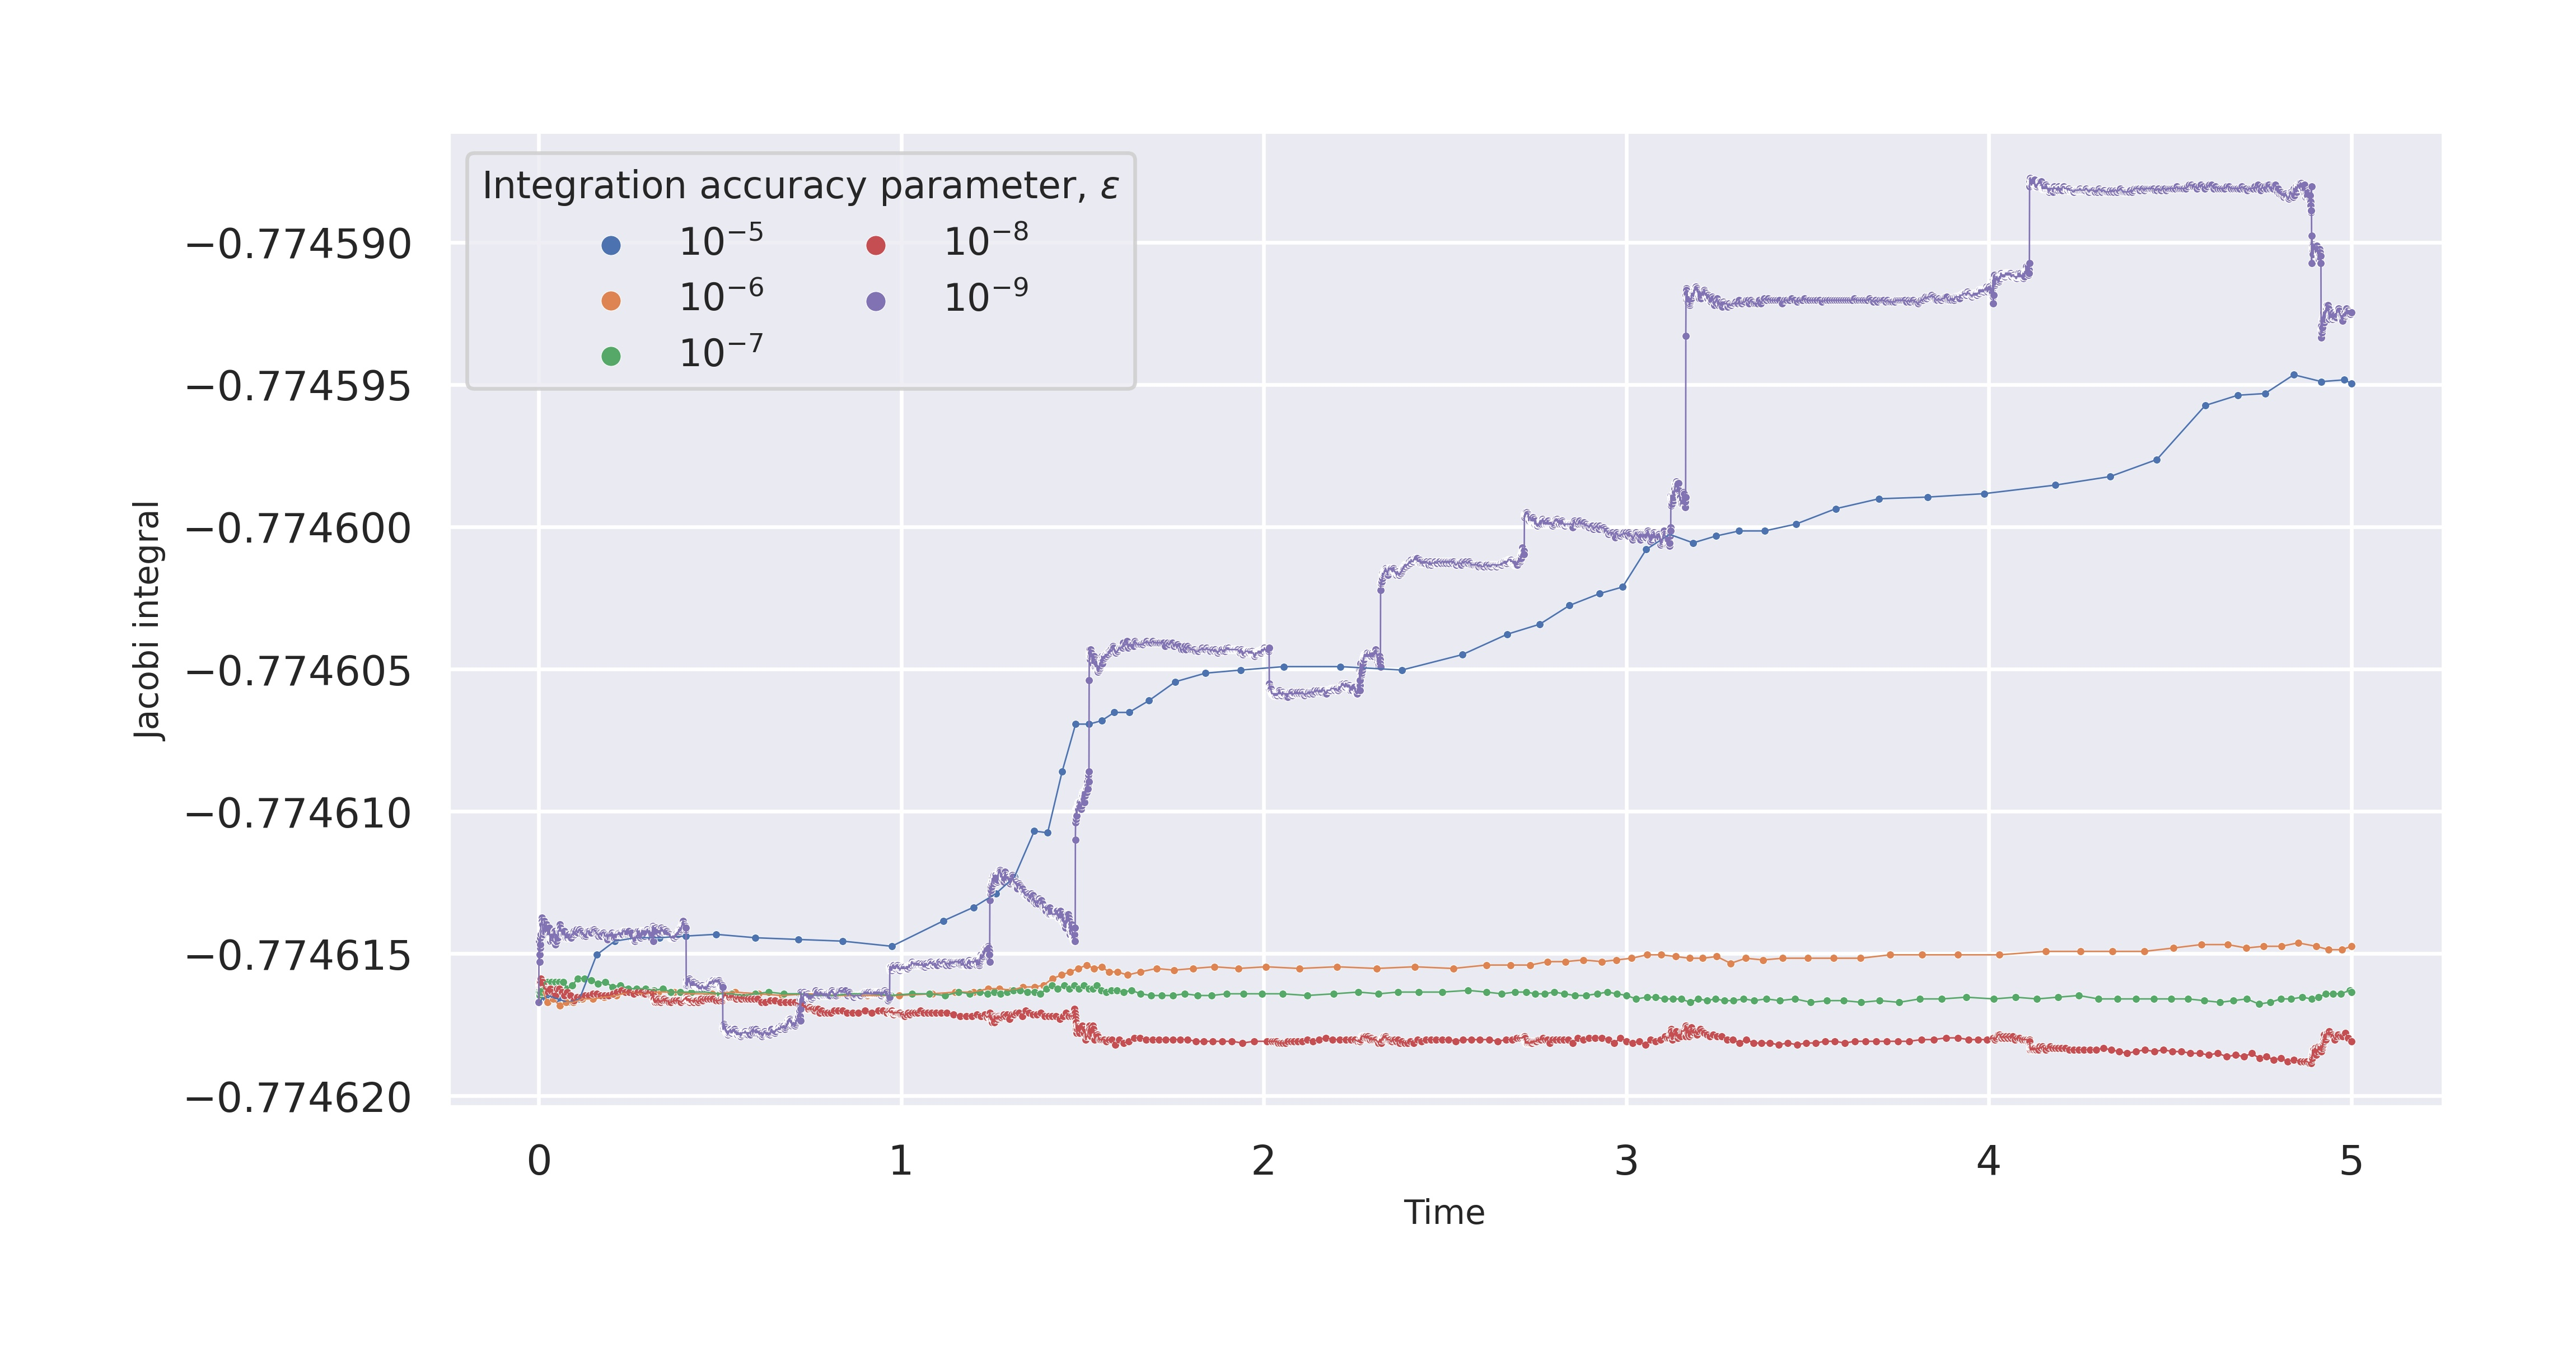
\includegraphics[width=\columnwidth]{../task1/q3-epsilon/plots/q3.jpg}
				\caption{Variation of Jacobi integral with time for different values of \(\epsilon\), a parameter that signifies the accuracy of integration.}
				\label{fig:task1.3}
			\end{figure}
			
			\begin{table} [h]
				\centering
				\setlength{\tabcolsep}{20pt} 
				\begin{tabular} {c c}
					\toprule
					\textbf{\(\epsilon\)} & \textbf{\(\sigma_{E_j}\)} \\
					\midrule
					\addlinespace
					\(10^{-5}\) & \(7.326 \times 10^{-6}\)
					\\ 
					\(10^{-6}\) & \(6.490 \times 10^{-7}\) \\
					\(10^{-7}\) & \(1.887 \times 10^{-7}\) \\
					\(10^{-8}\) & \(6.918 \times 10^{-7}\) \\
					\(10^{-9}\) & \(1.013 \times 10^{-5}\) \\
					\bottomrule
				\end{tabular}
				\caption{Standard deviation \((\sigma_{E_j})\) in values of Jacobi Integral for different values of integration accuracy parameter \((\epsilon)\). }
				\label{table:task1.3}
			\end{table}
			
			\item The trajectories for a star with initial parameters defined in section \ref{methods1}, for final times of 5.0 and 20.0 in simulation are plotted in figure \ref{fig:task1.4}. 
			
			\begin{figure} 
				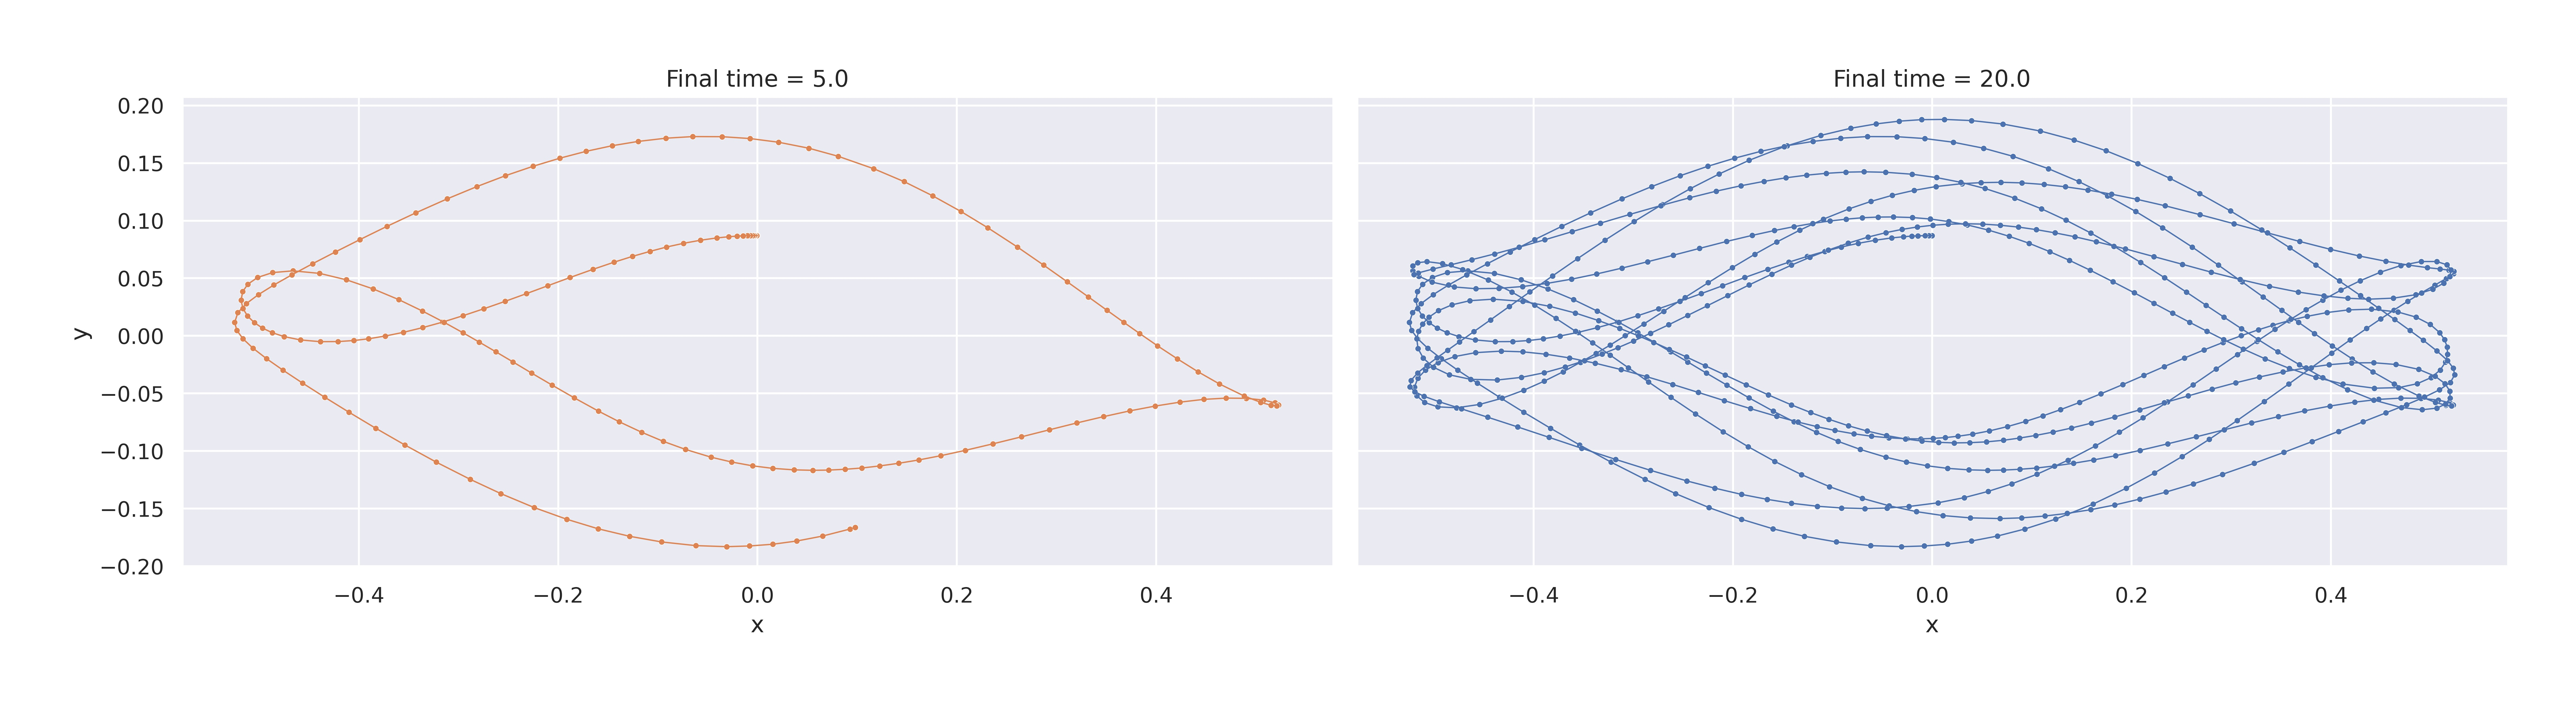
\includegraphics[width=\columnwidth]{../task1/q4-trajectory/plots/q4.jpg}
				\caption{Trajectories followed over (a) 5.0 units and (b) 20 units of time by a star with initial parameters, \((x,y)=(0,0.087)\) and \((v_x,v_y)=(-1.68,0)\).}
				\label{fig:task1.4}
			\end{figure}
			
			\item The calculated trajectories for a final time of 20.0 corresponding to initial values of \(v_x = \) -1.68, -1.64 and -1.635 are plotted for comparison in figure \ref{fig:task1.5}-(Top). The individual trajectories are plotted separately in figures \ref{fig:task1.4}(b) and \ref{fig:task1.5}-(Bottom). 
			
			\begin{figure} [h]
				
\includegraphics[width=\columnwidth]{../task1/q5q6-velocity/plots/q5_combined.jpg}
				\hrule
				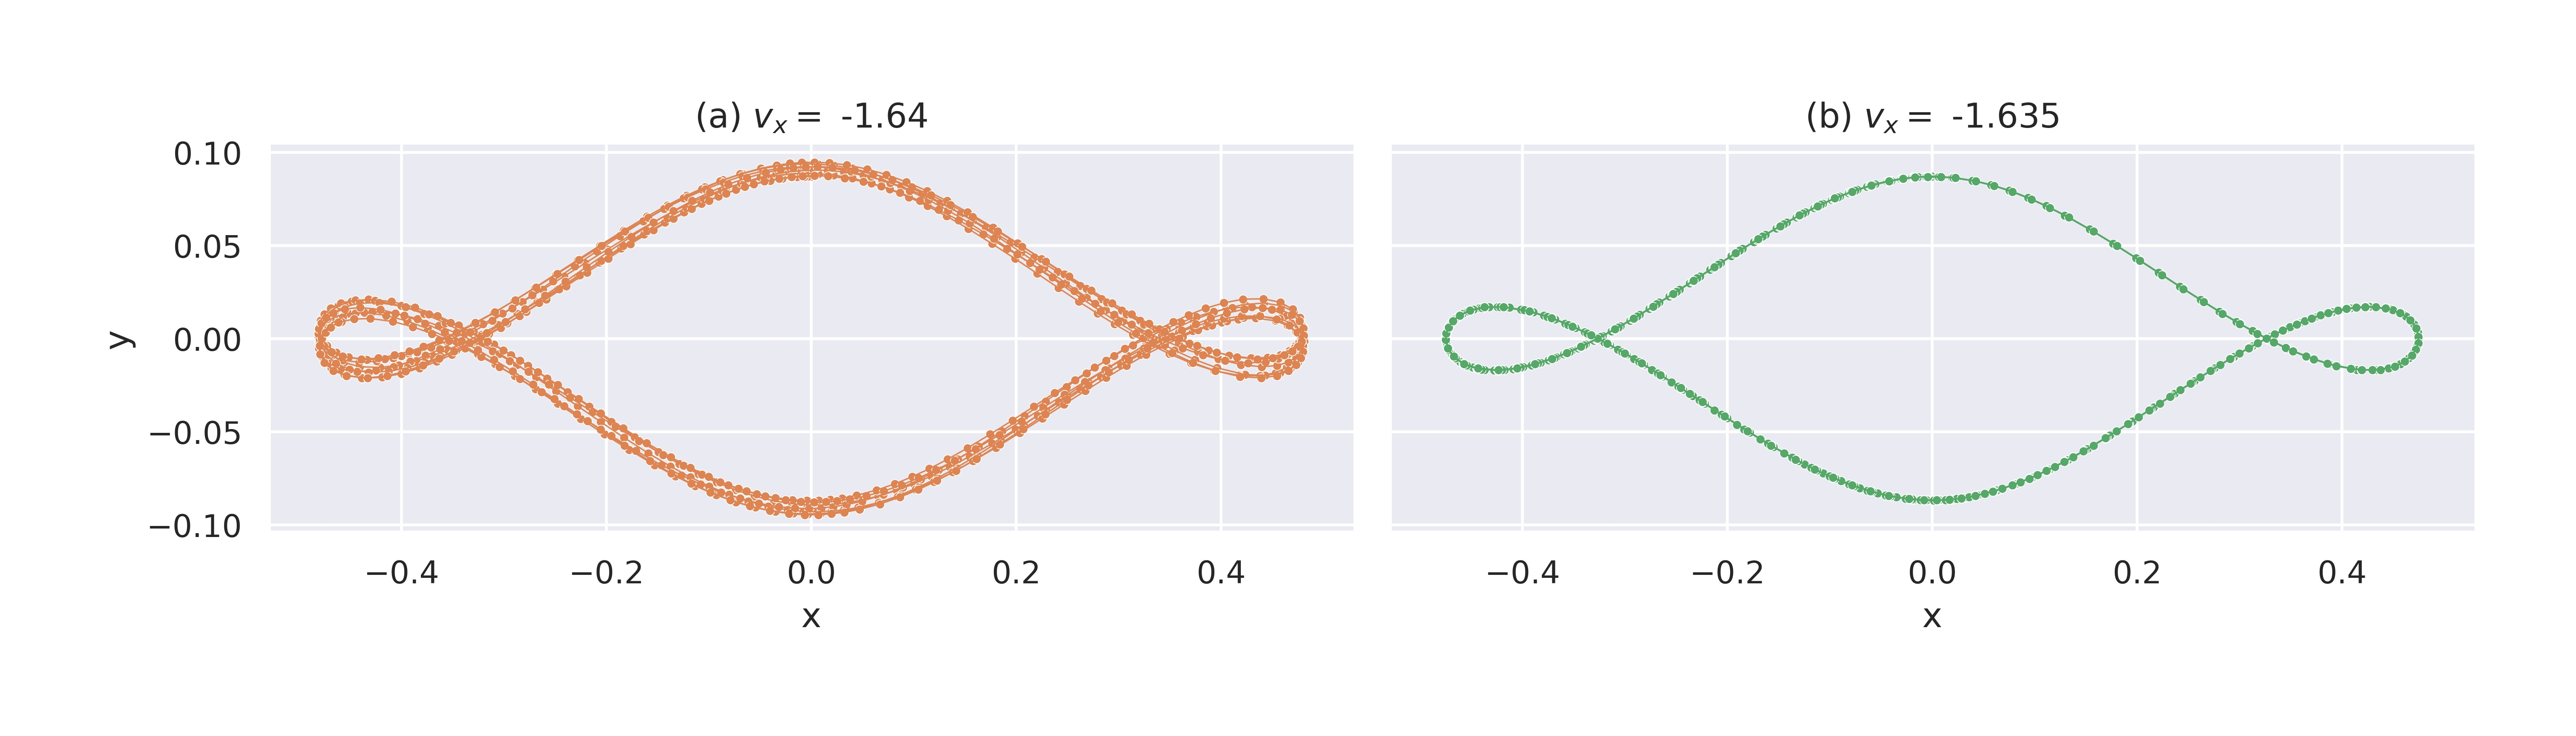
\includegraphics[width=\columnwidth]{../task1/q5q6-velocity/plots/q5_sep.jpg}
				\caption{(Top) A comparison plot showing trajectories followed by a star for different initial values of \(v_x\). (Bottom \(1 \times 2\) grid) Trajectories followed by a star for initial values of \(v_x\) equal to (a) -1.64, and (b) -1.635 shown separately. Note that the trajectory for \(v_x = -1.68\) is shown individually in figure \ref{fig:task1.4}(b). }
				\label{fig:task1.5}
			\end{figure}
			
			\item Similar plots for initial values of \(v_x = \) -1.63, -1.58, -1.15, -0.6, -0.524 and -0.4 are plotted for comparison in figure \ref{fig:task1.6}-(Top) and separately in figure \ref{fig:task1.6}-(Bottom).
			
			\begin{figure} [h]
				\includegraphics[width=\columnwidth]{../task1/q5q6-velocity/plots/q6_combined.jpg}
				\hrule
				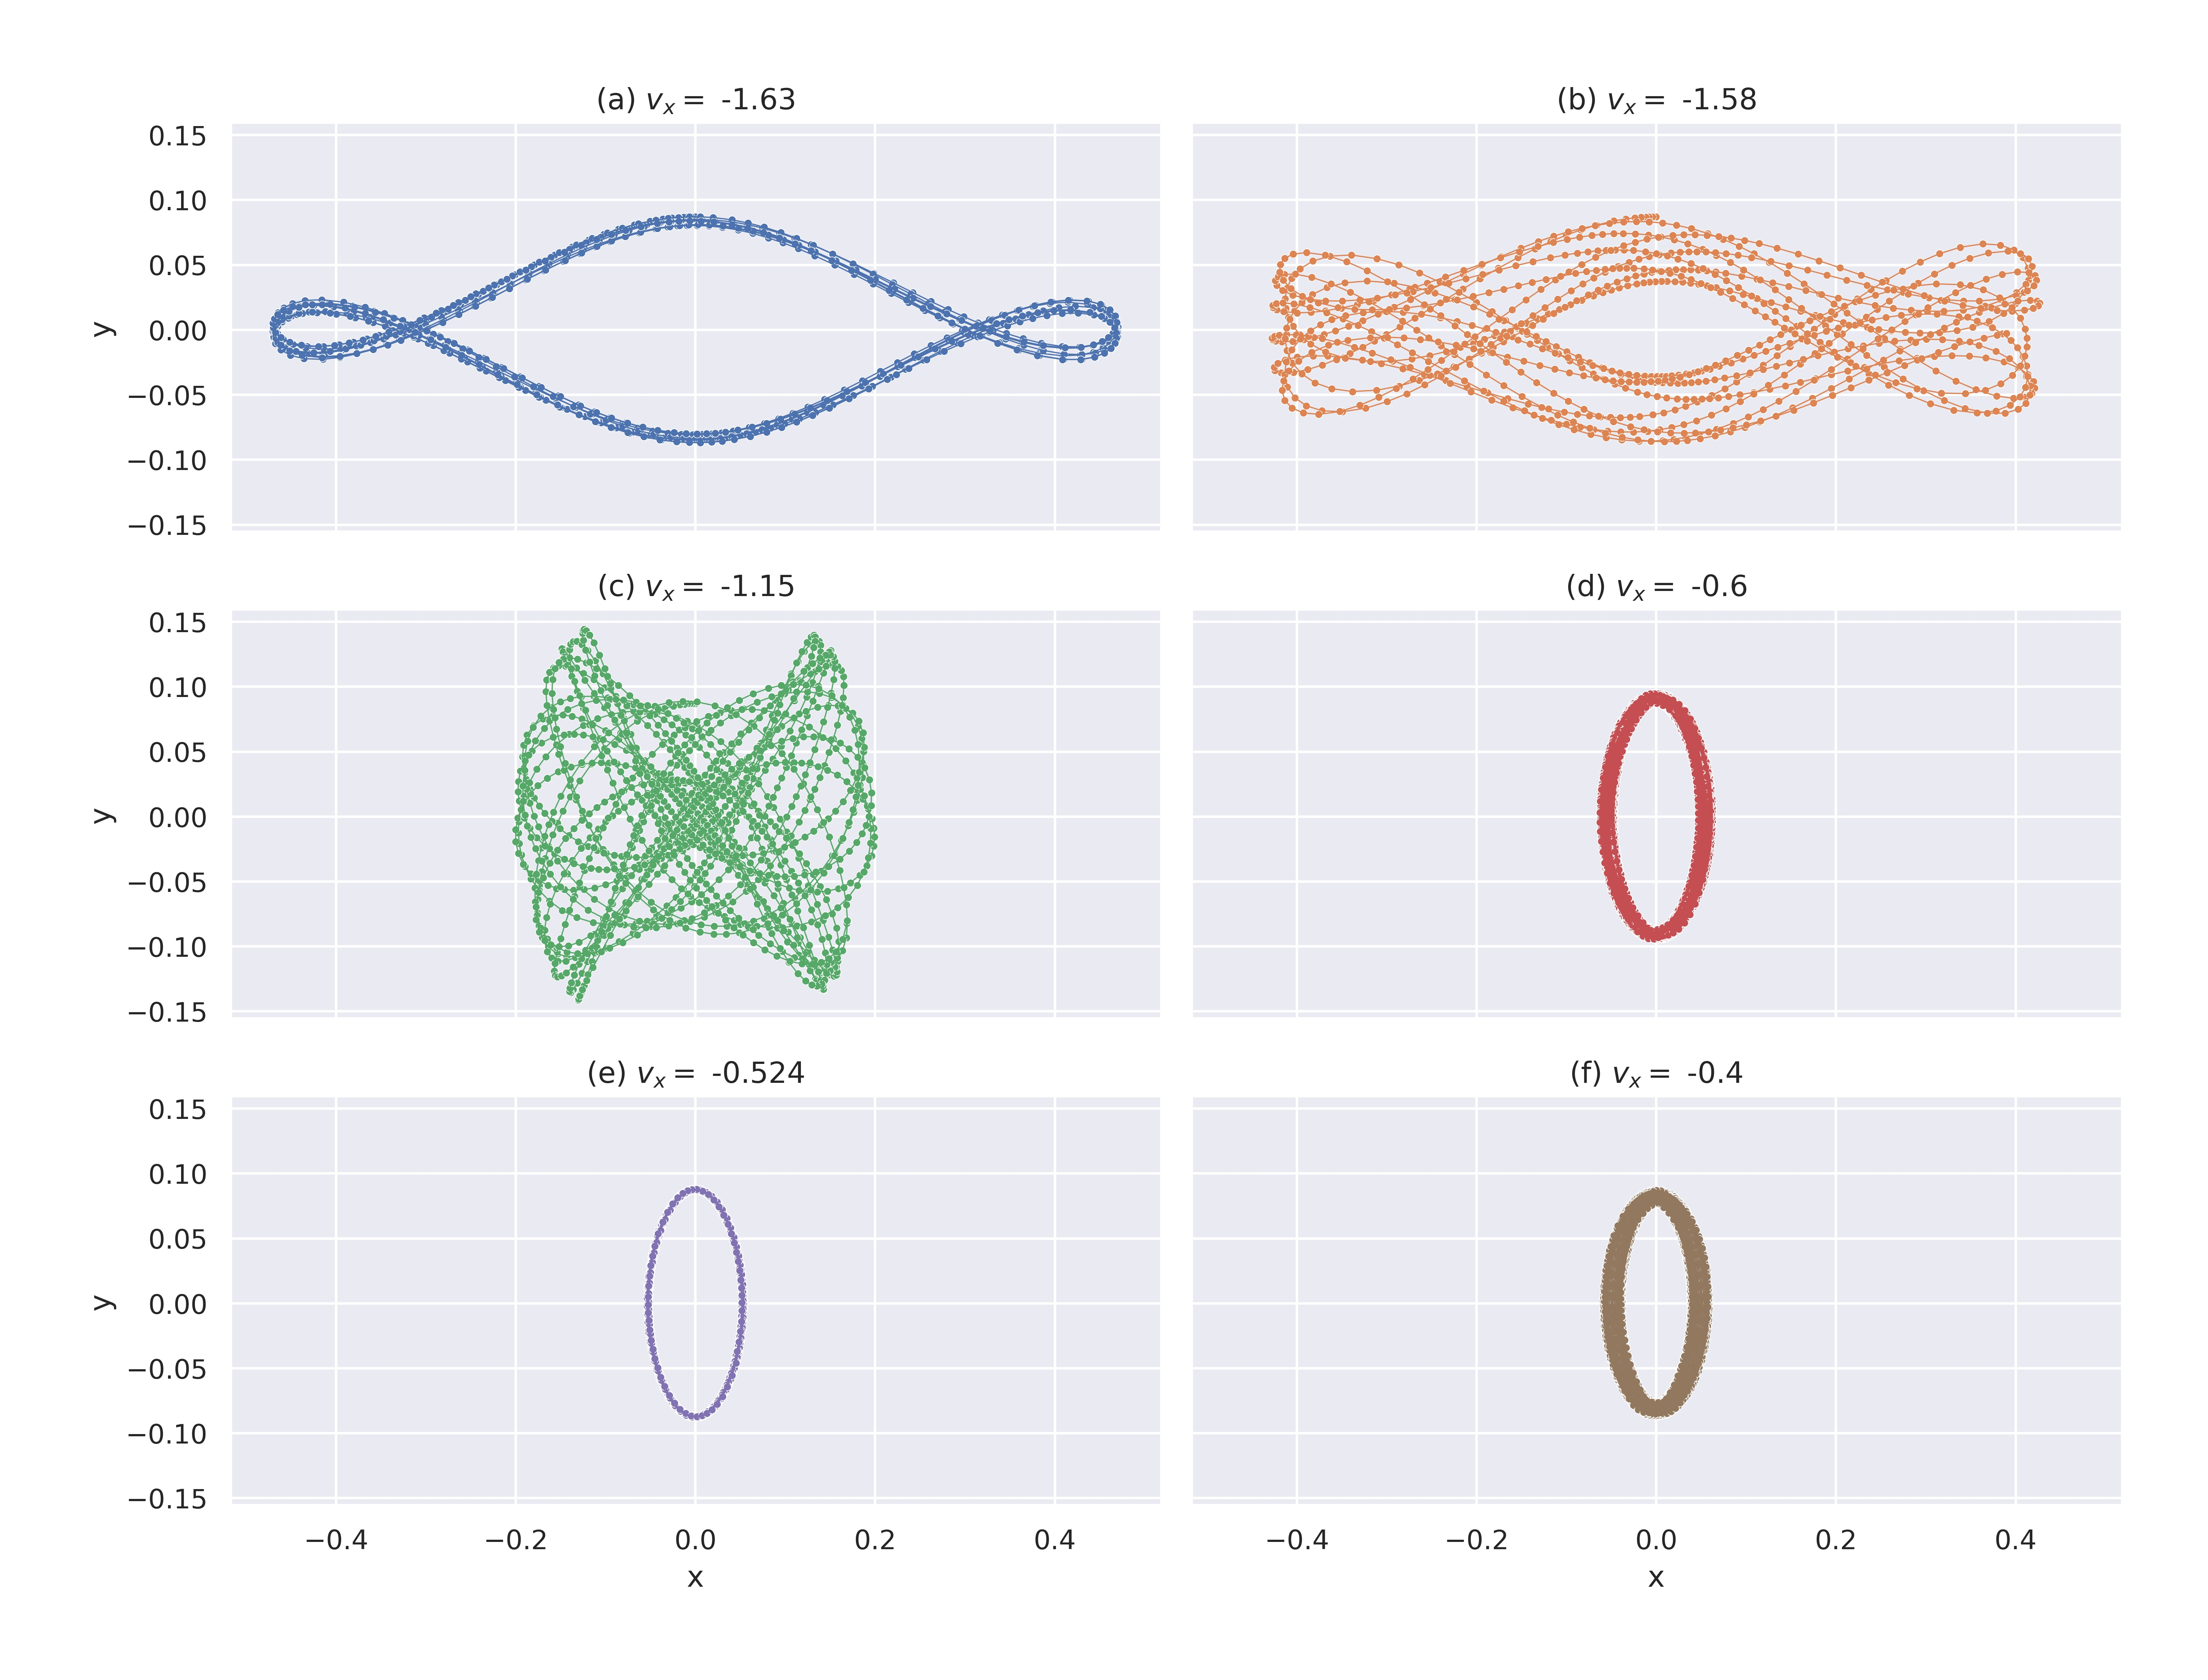
\includegraphics[width=\columnwidth]{../task1/q5q6-velocity/plots/q6_sep.jpg}
				\caption{(Top) A comparison plot showing trajectories followed by a star for different initial values of \(v_x\). (Bottom \(3 \times 2\) grid) Trajectories followed by a star for initial values of \(v_x\) equal to (a) -1.63, (b) -1.58, (c) -1-15, (d) -0.6, (e) -0.524 and (f) -0.4 shown separately.}
				\label{fig:task1.6}
			\end{figure}
		\end{itemize}
		
	
		% ----------------------------Results -----------------------------------------------
		
		\subsection{Discussions} \label{discussions1}
		
		\begin{itemize}
			
			\item The accuracy of integration increases with reduction in time-step, although it increases execution time. However, below a certain value of integration accuracy parameter, \(\epsilon\), the accuracy tends to decrease, as seen in figure \ref{fig:task1.3}.
			
			\item The trajectory followed by the star with \(v_x = -1.635\) in figure \ref{fig:task1.5}(b) is a case of \emph{stable periodic orbit}. Such an orbit has a closed geometry and the motion repeats after a fixed interval of time.
			
			\item Slight variation in the parameters from the case of \(v_x = -1.635\), we get trapped orbits. Examples of such orbits are  for \(v_x = -1.64\) and \(-1.68\). A larger deviation in parameters from the stable periodic orbit leads to a less tightly bound trapped orbit, as in the case of \(v_x = -1.68\). Such orbits are neither periodic nor closed and tend to stay in the vicinity of the parent stable periodic orbit.
			
			\item Similar trend can be noted in figure \ref{fig:task1.6}, where the stable periodic orbit occurs at \(v_x = -0.524\) (figure \ref{fig:task1.6}(e)). A morphological transition in orbits can be seen as we move from one stable periodic orbit (\(v_x = -1.635\)) to another (\(v_x = -0.524\)). Accordingly, the orbit for \(v_x = -1.15\), for which the initial parameters deviate the most, from the two periodic stable orbits, ends up being the trapped orbit with most loosely bound morphology.
			
			\item With decrease in \(v_x\), we get orbits that are more tightly bound to the center of the potential well. This trend can be seen through the decreasing span of orbits along x-axis as we move to lower values of \(v_x\) in figures \ref{fig:task1.5} and \ref{fig:task1.6}. 
			
		\end{itemize}
		
	% ========================= Part 1 ======================================================
	
	\clearpage
	\section{Part 2 - Fourier Transform and Spectral Analysis} \label{task2}
	
		% ----------------------------Methods -----------------------------------------------
	
		\subsection{Methods} \label{methods2}
	
		% ----------------------------Results -----------------------------------------------
		
		\subsection{Results} \label{results2}
		
		\begin{figure} [h]
			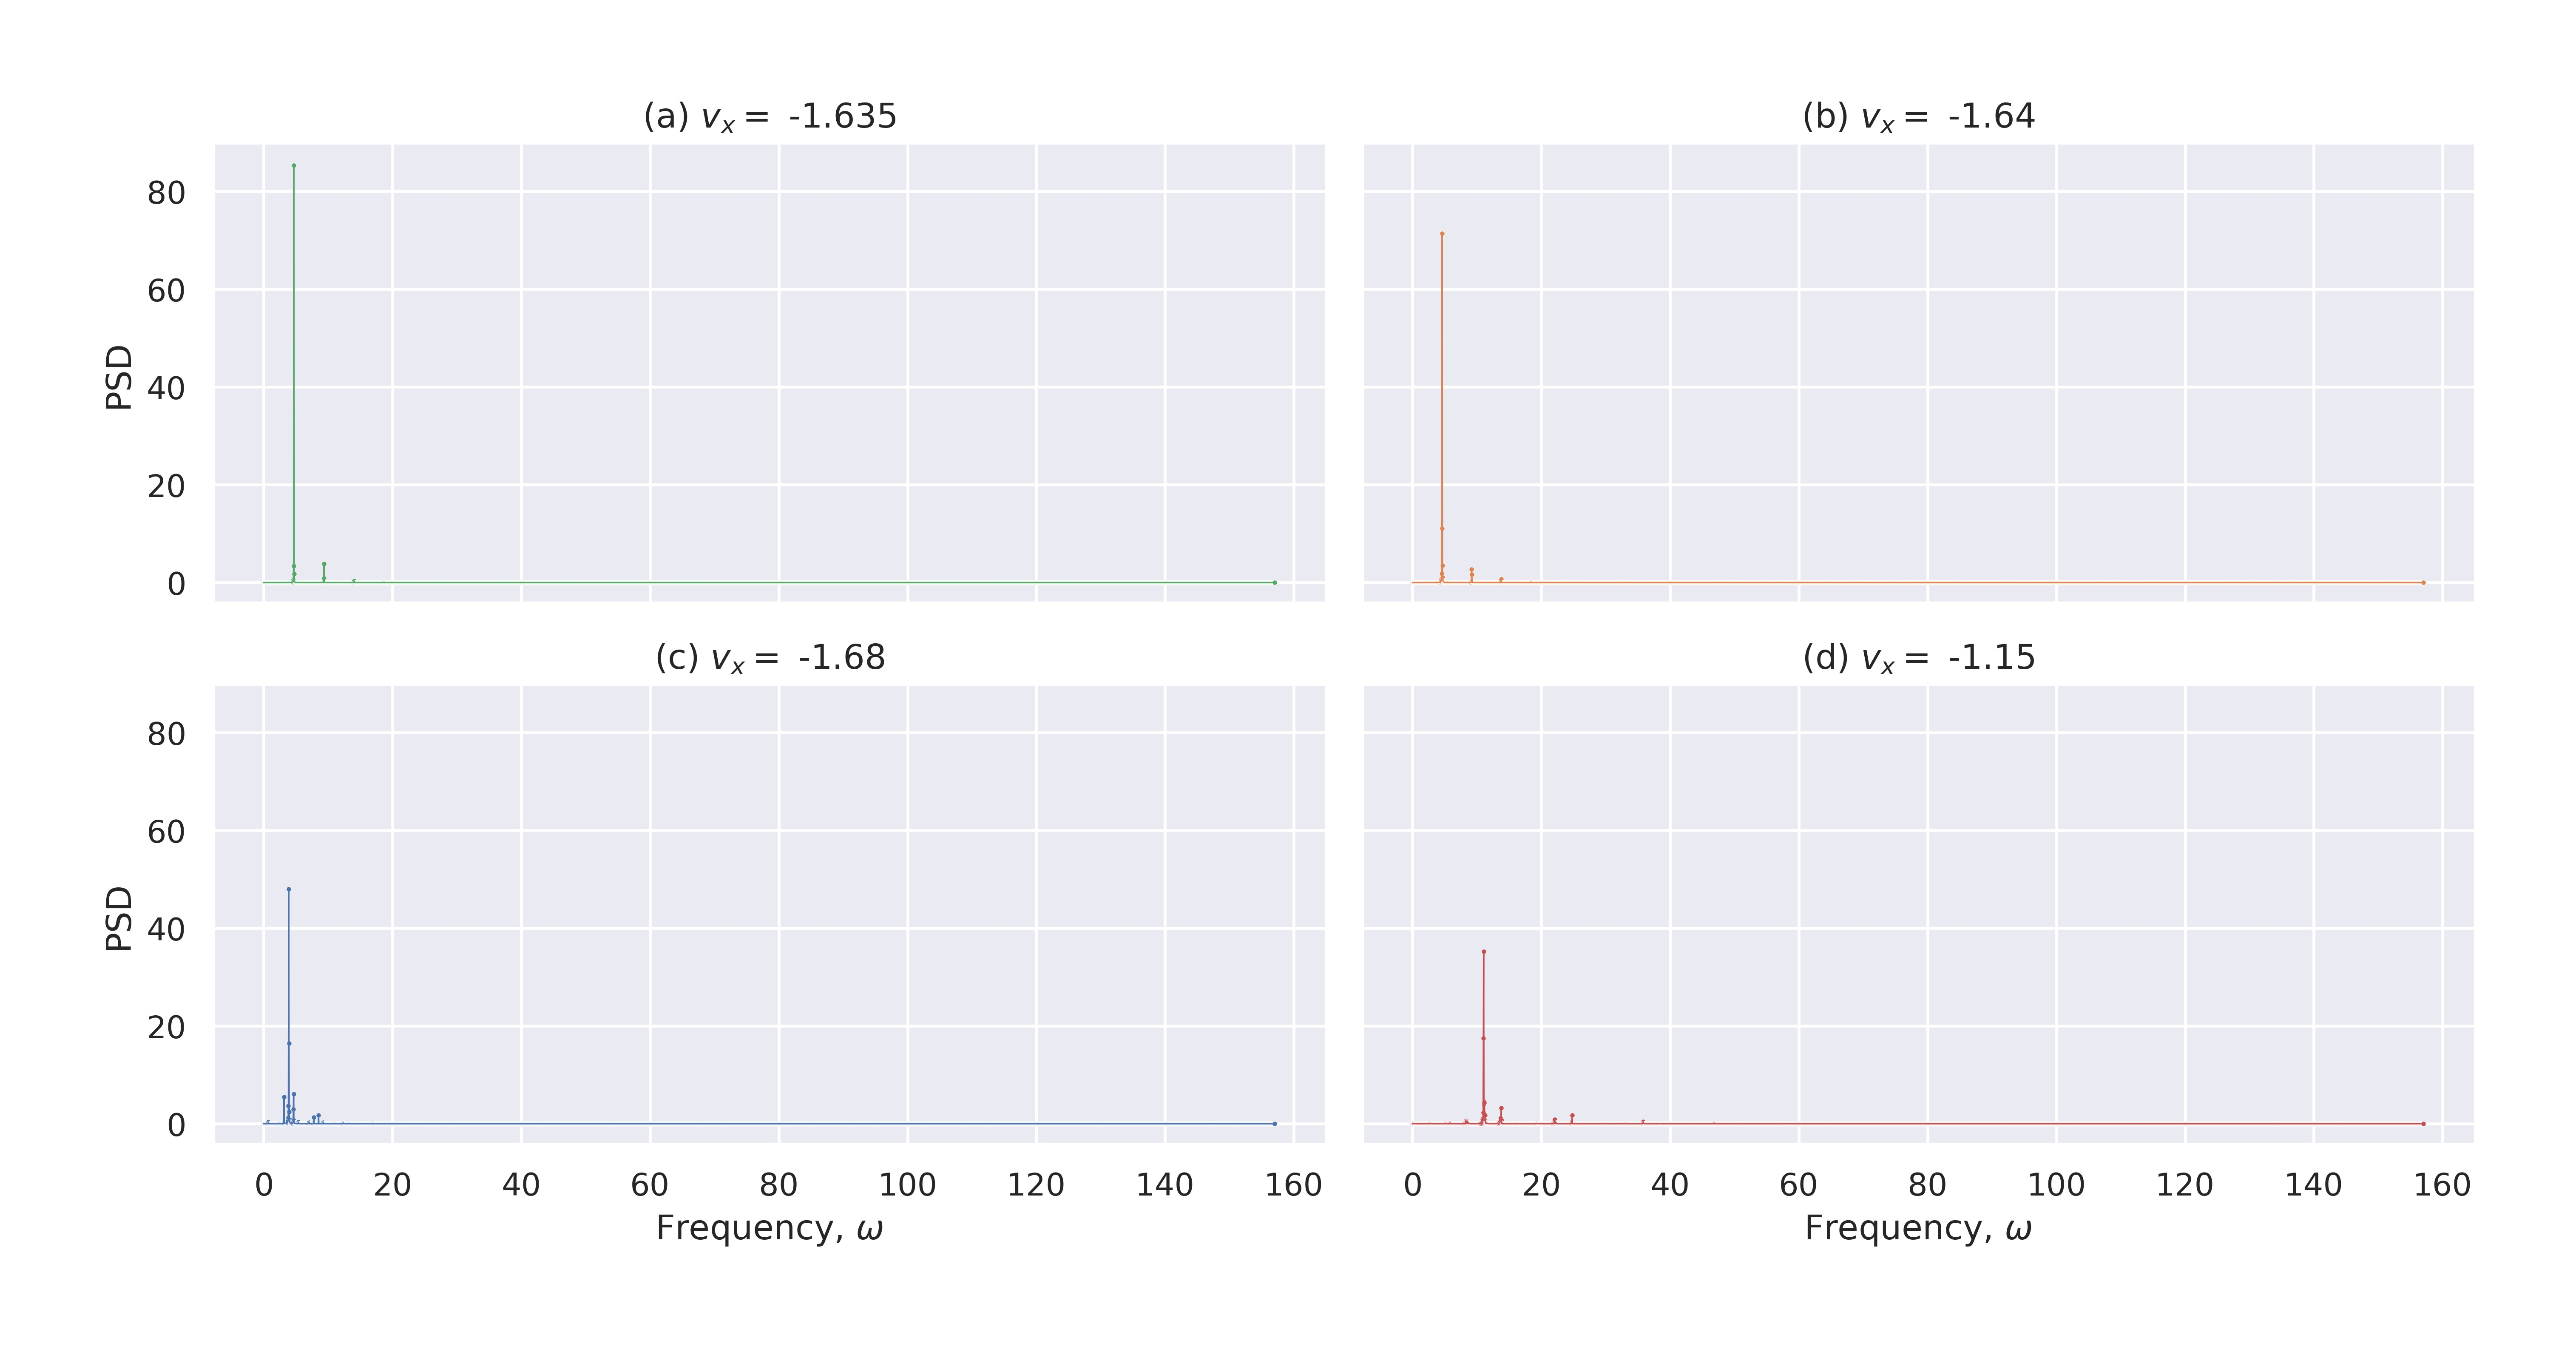
\includegraphics[width=\columnwidth]{../task2/plots/q1-5_lin.jpg}
			\caption{}
			\label{fig:task2_lin}
		\end{figure}
		
		\begin{figure} [h]
			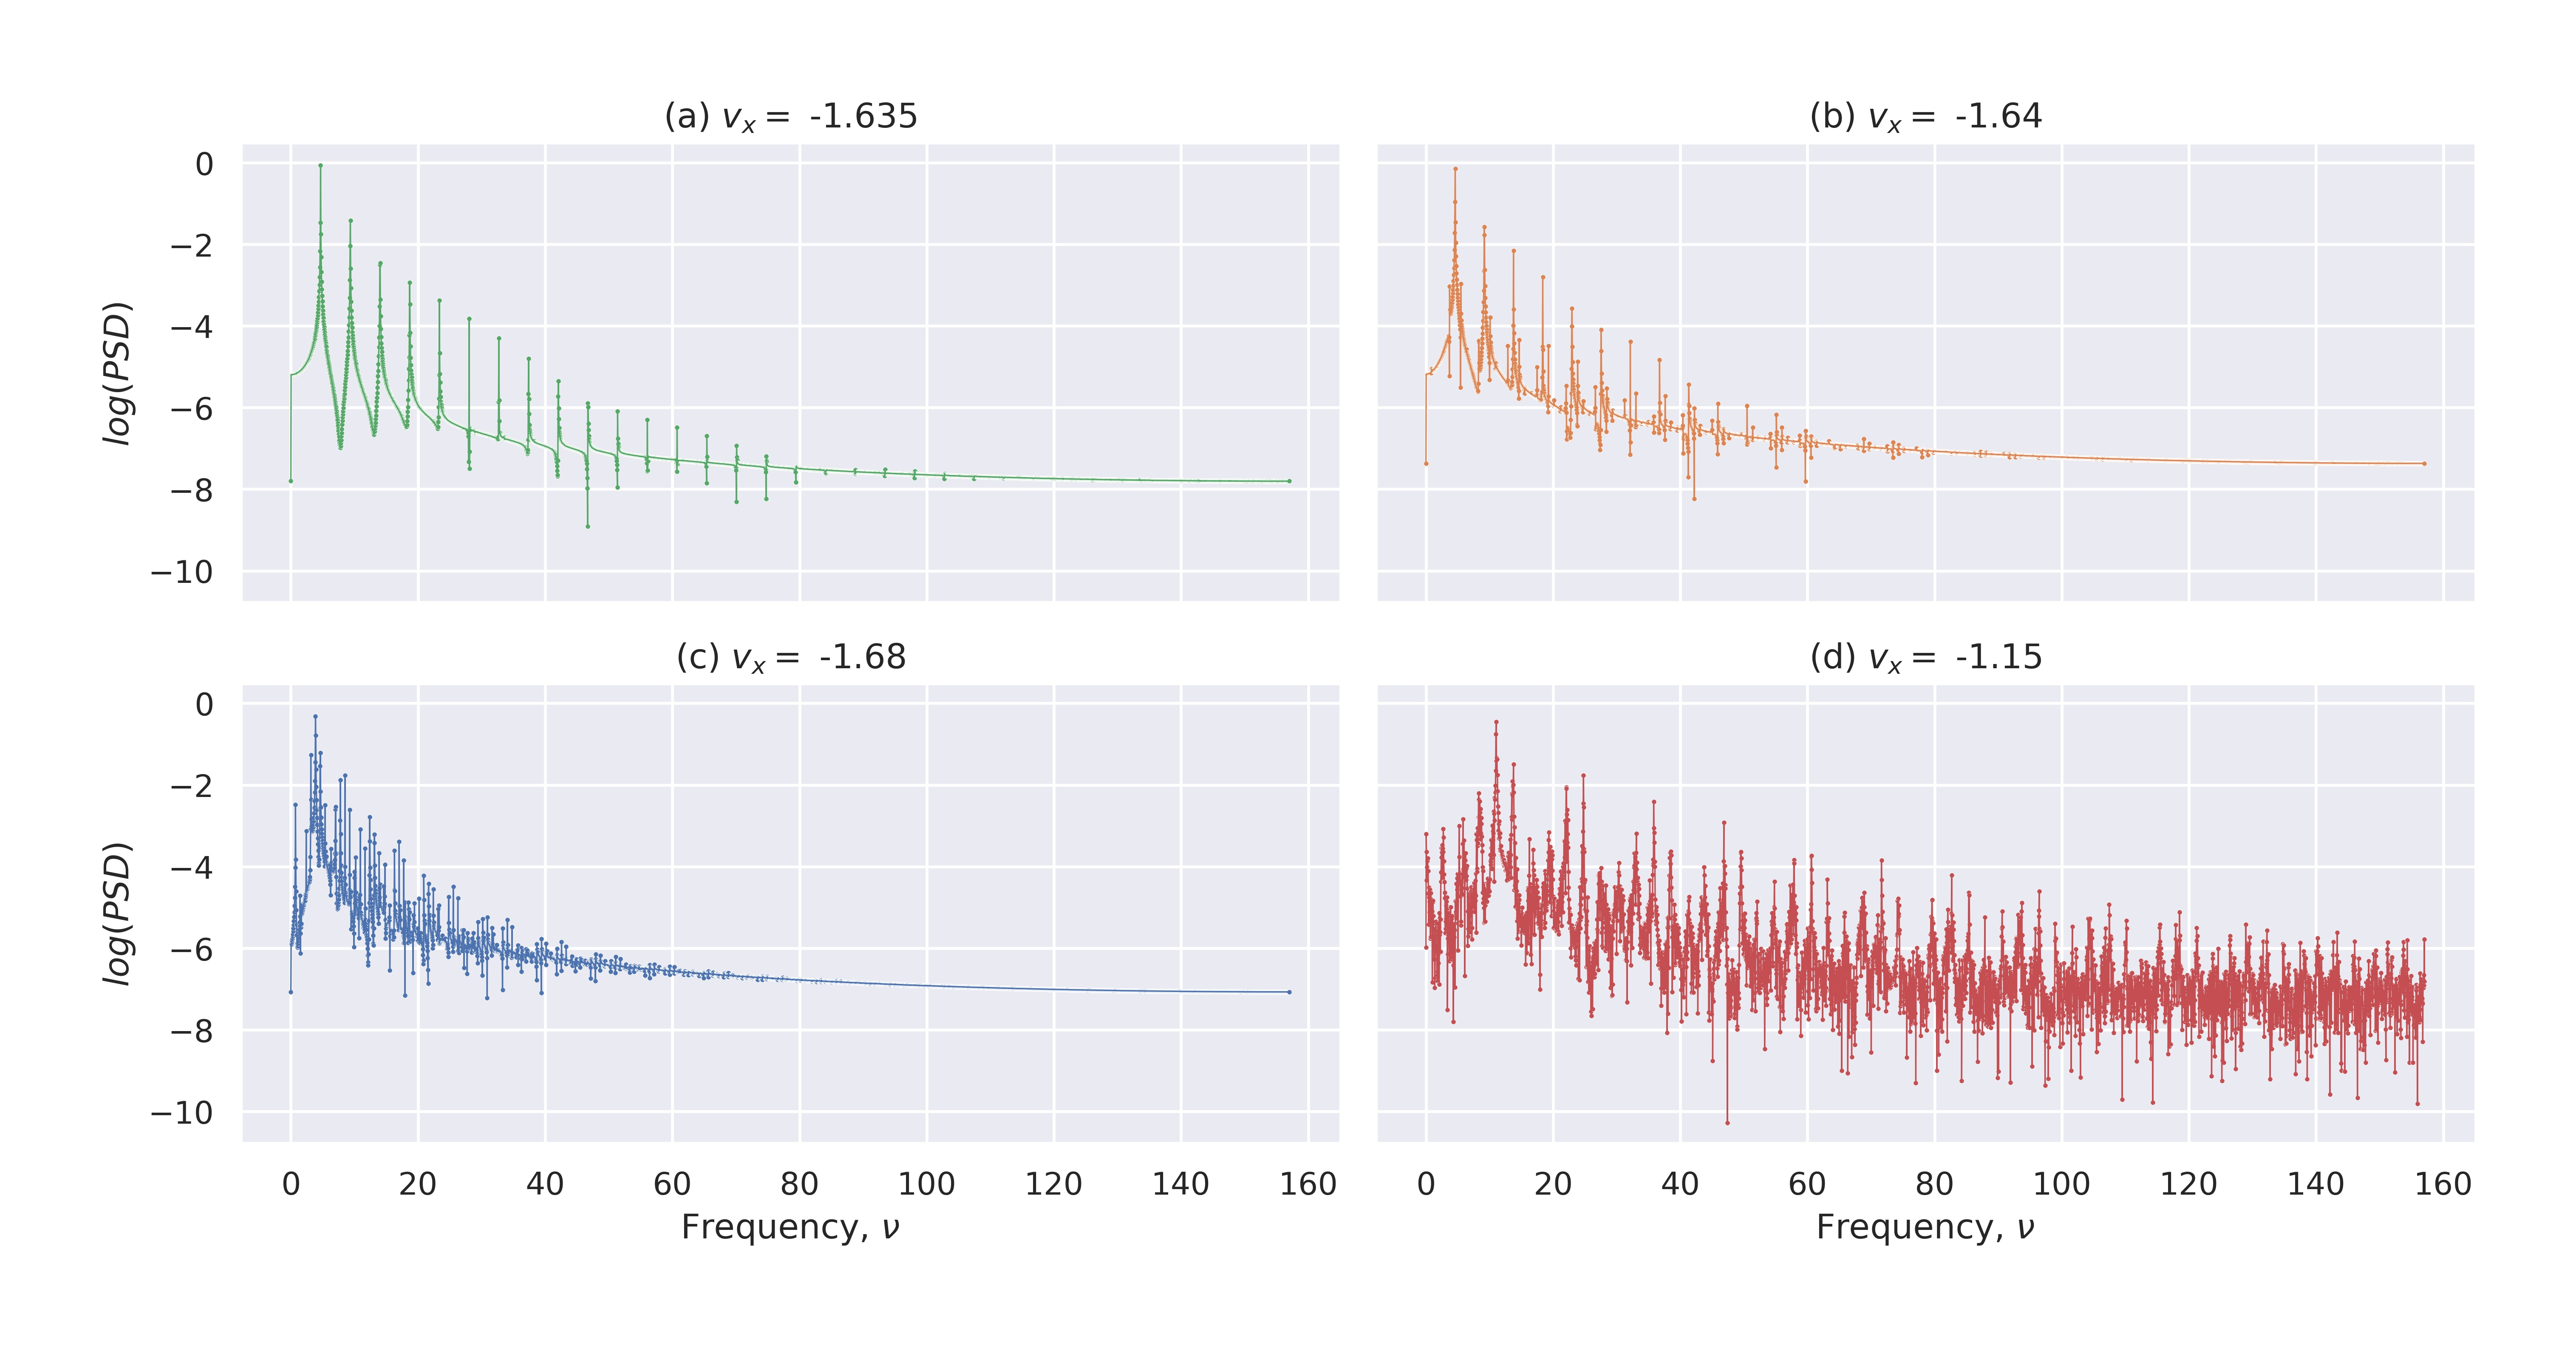
\includegraphics[width=\columnwidth]{../task2/plots/q1-5_log.jpg}
			\caption{}
			\label{fig:task2:log}
		\end{figure}
	
	
	% ========================= Conclusions =================================================
	
	\section{Conclusions} \label{conclusions}
	
	
\end{document}